\section{Convolution of linear function}

Given kernel, 
\[
h(t) =
\begin{cases}
1, & \text{for } -T \leq t \leq T \\
0, & \text{otherwise}
\end{cases}
\]
and the function 
\begin{align*}
f(t) &= at+b
\end{align*}
Let $y(t) = x(t) * f(t)$, then
\begin{align*}
	y(t) &= h(t) * f(t) \\
             &= f(t) * h(t) \\
             &= \int_{-\infty}^{\infty} f(\tau) h(t - \tau) d \tau \\
\end{align*}
\[
h(t - \tau) =
\begin{cases}
1, & \text{for } -T \leq t - \tau \leq T \\
0, & \text{otherwise}
\end{cases}
\]
\[
h(t - \tau) =
\begin{cases}
1, & \text{for } \tau - T \leq t \leq \tau + T \\
0, & \text{otherwise}
\end{cases}
\]
Therefore, the convolution becomes, 
\begin{align*}
	y(t) &= \int_{t - T}^{t + T} (at+b)* 1 d\tau \\
	y(t) &= \int_{t - T}^{t + T}  (at+b)d\tau\\
    y(t) &= \frac{a}{2}[(t+T)^2-(t-T)^2]+b[t+T-(t-T)]\\
    y(t) &= 2atT+2bT
\end{align*}
This integration can be numerically computed and can be seen to be the following - (we are using the values of  and b as 1)\\
\newpage
For different values of T, the change in $y(t)$ is depicted in the following - \\
\begin{figure}[h]
    \centering
    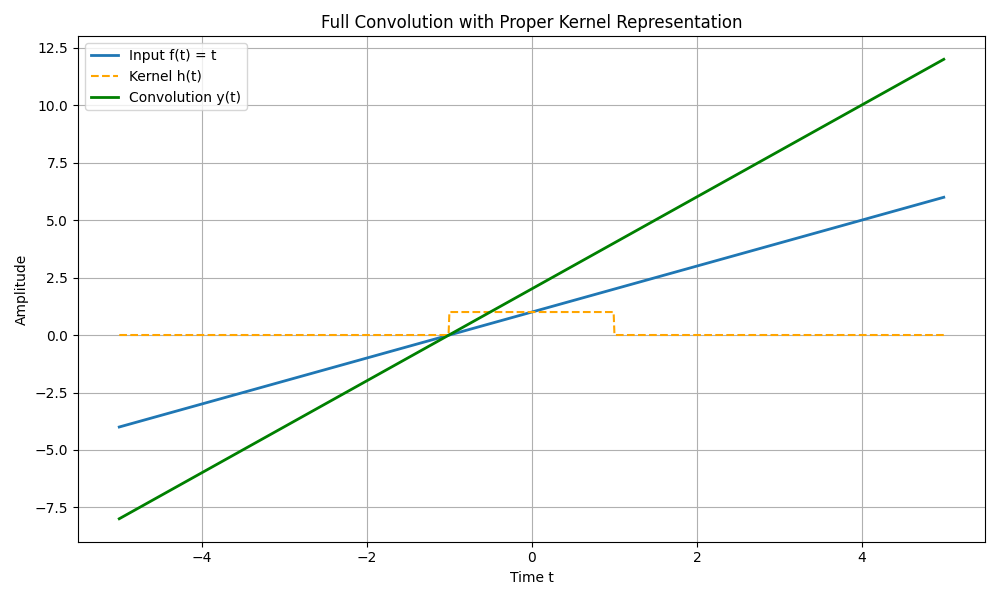
\includegraphics[width=0.6\textwidth]{figsm/1.png}
    \caption{T = 1}
    \label{fig:conv_sinc}
\end{figure}
\begin{figure}[h]
    \centering
    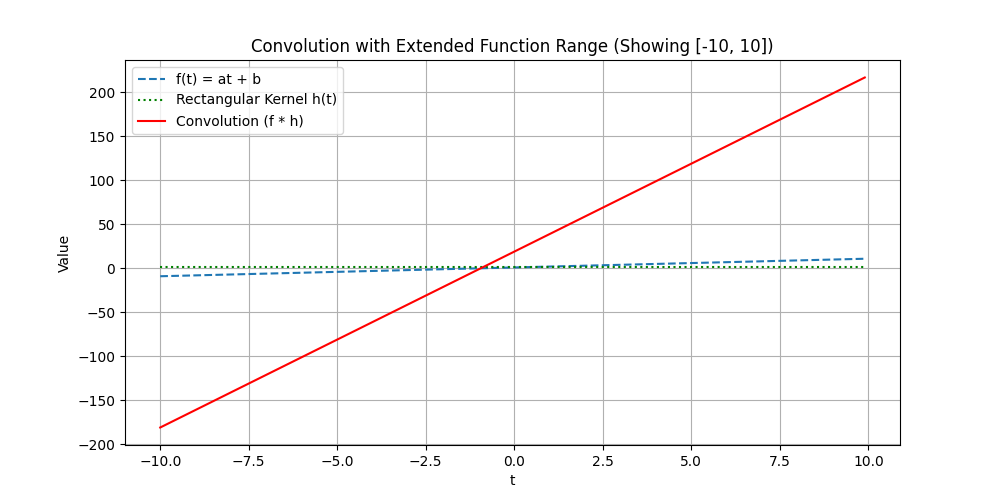
\includegraphics[width=0.6\textwidth]{figsm/2.png}
    \caption{T = 1}
    \label{fig:conv_sinc}
\end{figure}
It can be seen that as $T$ increases, the slope of the output is increasing but it is still linear.
\newpage
\subsection{Considering the kernel for $t>0$}
The response of the system for different values of $T$ are as follows -\\
Modified kernel is, 
\[
h(t) =
\begin{cases}
1, & \text{for} 0 \leq t \leq T \\
0, & \text{otherwise}
\end{cases}
\]
and the function 
\begin{align*}
f(t) &= at+b
\end{align*}
Let $y(t) = x(t) * f(t)$, then
\begin{align*}
	y(t) &= h(t) * f(t) \\
             &= f(t) * h(t) \\
             &= \int_{-\infty}^{\infty} f(\tau) h(t - \tau) d \tau \\
\end{align*}
\[
h(t - \tau) =
\begin{cases}
1, & \text{for } 0 \leq t - \tau \leq T \\
0, & \text{otherwise}
\end{cases}
\]
\[
h(t - \tau) =
\begin{cases}
1, & \text{for } \tau - T \leq t \leq \tau \\
0, & \text{otherwise}
\end{cases}
\]
Therefore, the convolution becomes, 
\begin{align*}
	y(t) &= \int_{t - T}^{t + T} (at+b)* 1 d\tau \\
	y(t) &= \int_{t - T}^{t + T}  (at+b)d\tau\\
    y(t) &= \frac{a}{2}[(t)^2-(t-T)^2]+b[t-(t-T)]\\
    y(t) &= atT-\frac{a}{2}{T}^2+bT
\end{align*}
\begin{figure}[h]
    \centering
    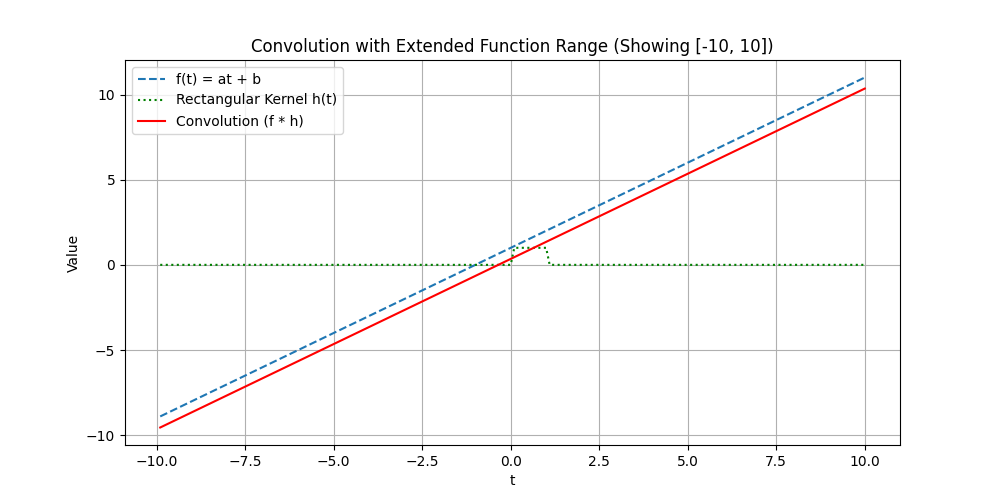
\includegraphics[width=0.6\textwidth]{figsm/3.png}
    \caption{T = 1,A=1,B=1}
    \label{fig:conv_sinc}
\end{figure}
\begin{figure}[h]
    \centering
    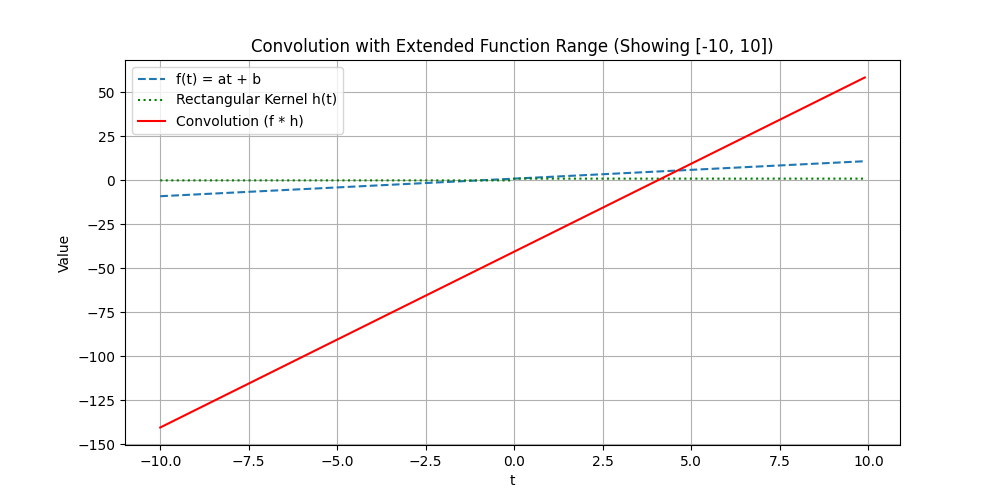
\includegraphics[width=0.6\textwidth]{figsm/4.png}
    \caption{T = 10,A=1,B=1}
    \label{fig:conv_sinc}
\end{figure}
\newpage

\subsection{Shifting the kernel by $t_{0}$}
Shifting of kernel means moving the kernel to the left or right by an amount, i.e., if the given kernel is shifted by an amount $t_0$, then it becomes, 
\[
h(t) =
\begin{cases}
1, & \text{for } -T \leq t-t_0 \leq T \\
0, & \text{otherwise}
\end{cases}
\]
\[
h(t) =
\begin{cases}
1, & \text{for } -T+t_0 \leq t \leq T+t_0 \\
0, & \text{otherwise}
\end{cases}
\]
\begin{align*}
f(t) &= at+b
\end{align*}
Let $y(t) = x(t) * f(t)$, then
\begin{align*}
	y(t) &= h(t) * f(t) \\
             &= f(t) * h(t) \\
             &= \int_{-\infty}^{\infty} f(\tau) h(t - \tau) d \tau \\
\end{align*}
\[
h(t - \tau) =
\begin{cases}
1, & \text{for } -T+t_0 \leq t - \tau \leq T+t_0 \\
0, & \text{otherwise}
\end{cases}
\]
\begin{align*}
	y(t) &= \int_{t - T}^{t + T} (at+b)* 1 d\tau \\
	y(t) &= \int_{t - T}^{t + T}  (at+b)d\tau\\
    y(t) &= \frac{a}{2}[(t)^2-(t-T)^2]+b[t-(t-T)]\\
    y(t) &= 2a(t-t_0)T+2bT
\end{align*}

Here we can observe that the solution is shifted by 
$t_0$ as the kernel is shifted by $t_0=10$ for the case where T=A=B=1,
\begin{figure}[h]
    \centering
    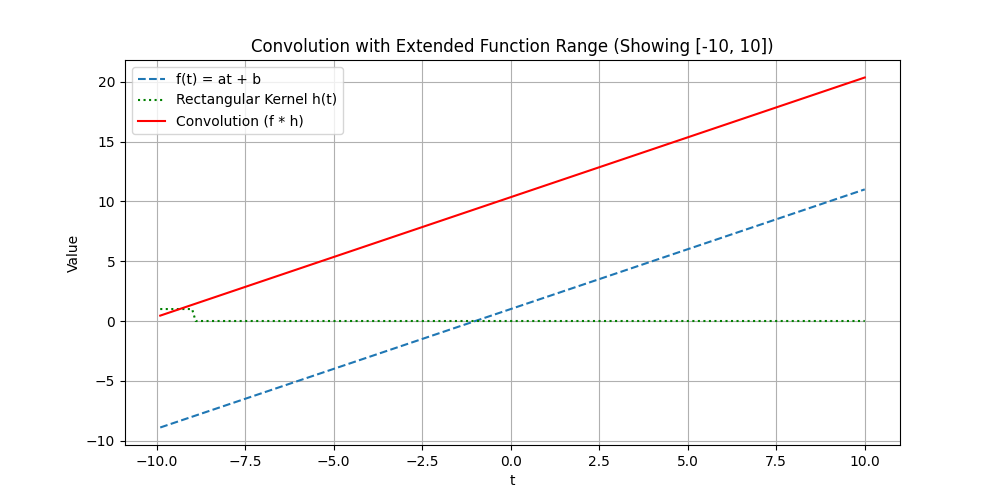
\includegraphics[width=0.6\textwidth]{figsm/5.png}
    \caption{$t_0 = 10$}
    \label{fig:conv_sinc}
\end{figure}
\begin{figure}[h]
    \centering
    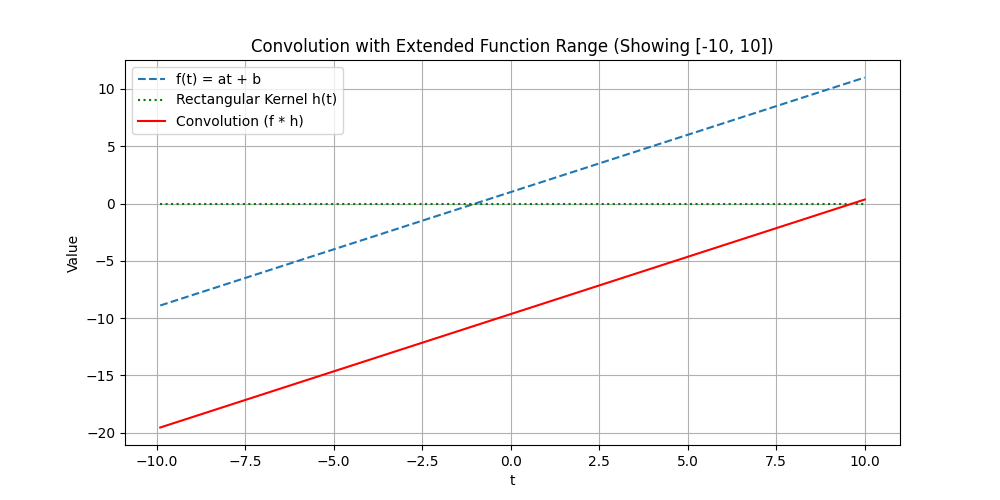
\includegraphics[width=0.6\textwidth]{figsm/6.png}
    \caption{$t_0 = -10$}
    \label{fig:conv_sinc}
\end{figure}
Shifting of the kernel by 10 units results in shifting of convoluted function by 10 units.
